% ICAART 2027 — revisão de 2026-09-13; versão enxuta de 2026-09-18 (a completa está em versoes/).
% Compilar com o template SCITEPRESS (SCITEPRESS.sty + apalike.bst), p.ex. no Overleaf.
% Números: todos vêm de tables/macros.tex e tables/*.tex, gerados por
%   python study/analysis/form_agreement.py   (RQ1–RQ3)
%   python study/analysis/benchmark.py        (RQ4: benchmark_macros, benchmark, benchmark_fig)
% Não digitar número à mão. Pendências do autor aparecem em vermelho (\TODO).

\documentclass[a4paper,twoside]{article}

\usepackage{epsfig}
\usepackage{subcaption}
\usepackage{calc}
\usepackage{amssymb}
\usepackage{amstext}
\usepackage{amsmath}
\usepackage{amsthm}
\usepackage{multicol}
\usepackage{pslatex}
\usepackage{apalike}
\usepackage{booktabs}
\usepackage{tabularx}
\usepackage{adjustbox}
\usepackage{url}
\usepackage{xcolor}
\usepackage{tikz}
\usetikzlibrary{arrows.meta,positioning,calc,shapes.geometric}
\usepackage{pgfplots}
\pgfplotsset{compat=1.18}
\usepgfplotslibrary{groupplots}
\usepackage{SCITEPRESS} % other packages must be loaded BEFORE SCITEPRESS.sty

% Reserva: o SCITEPRESS.sty oficial define estes comandos. Se o projeto não
% estiver usando o .sty do template, isto evita "Undefined control sequence"
% no bloco de autores. Com o .sty certo, \providecommand não faz nada.
\providecommand{\authorname}[1]{#1\\}
\providecommand{\affiliation}[1]{\textit{#1}\\}
\providecommand{\email}[1]{\textit{#1}}
\providecommand{\sup}[1]{$^{#1}$}
\providecommand{\orcidAuthor}[1]{}

\newcommand{\TODO}[1]{\textcolor{red}{[TODO: #1]}}
% GERADO por study/analysis/form_agreement.py — não editar à mão.
\newcommand{\NRaters}{18}
\newcommand{\NPosts}{10}
\newcommand{\NCHperDim}{180}
\newcommand{\NHHperDim}{1,530}
\newcommand{\HHexAll}{28.4\%}
\newcommand{\HHwAll}{68.7\%}
\newcommand{\CHexAll}{31.8\%}
\newcommand{\CHwAll}{78.6\%}
\newcommand{\CHchanceExAll}{31.9\%}
\newcommand{\CHchanceWAll}{78.4\%}
\newcommand{\ConstExAll}{39.2\%}
\newcommand{\ConstWAll}{86.5\%}
\newcommand{\CHexLo}{22.8\%}
\newcommand{\CHexHi}{40.8\%}
\newcommand{\CHwLo}{66.9\%}
\newcommand{\CHwHi}{88.2\%}
\newcommand{\HHexLo}{21.0\%}
\newcommand{\HHexHi}{36.5\%}
\newcommand{\HHwLo}{55.2\%}
\newcommand{\HHwHi}{81.0\%}
\newcommand{\DiffExLo}{$-$6.9}
\newcommand{\DiffExHi}{+10.5}
\newcommand{\DiffWLo}{+0.0}
\newcommand{\DiffWHi}{+17.4}
\newcommand{\ChanceDiffExLo}{$-$3.2}
\newcommand{\ChanceDiffExHi}{+3.0}
\newcommand{\ChanceDiffWLo}{$-$2.0}
\newcommand{\ChanceDiffWHi}{+2.6}
\newcommand{\HHchanceExAll}{28.8\%}
\newcommand{\HHchanceWAll}{69.0\%}
\newcommand{\HHChanceDiffExLo}{$-$5.5}
\newcommand{\HHChanceDiffExHi}{+1.3}
\newcommand{\HHChanceDiffWLo}{$-$3.7}
\newcommand{\HHChanceDiffWHi}{+1.2}
\newcommand{\HumMeanCla}{3.91}
\newcommand{\CriMeanCla}{4.00}
\newcommand{\BiasCla}{+0.09}
\newcommand{\BiasLoCla}{$-$0.26}
\newcommand{\BiasHiCla}{+0.48}
\newcommand{\MAECla}{0.76}
\newcommand{\KappaCla}{0.00}
\newcommand{\RhoCla}{n/a}
\newcommand{\AlphaCla}{$-$0.02}
\newcommand{\AlphaLoCla}{$-$0.05}
\newcommand{\AlphaHiCla}{$-$0.01}
\newcommand{\CHexCla}{41.1\%}
\newcommand{\HHexCla}{31.7\%}
\newcommand{\CriDistinctCla}{1}
\newcommand{\PostMeanSDCla}{0.21}
\newcommand{\HumModeCla}{4}
\newcommand{\VarPostCla}{3\%}
\newcommand{\VarRaterCla}{43\%}
\newcommand{\HumMeanRel}{3.74}
\newcommand{\CriMeanRel}{3.20}
\newcommand{\BiasRel}{$-$0.54}
\newcommand{\BiasLoRel}{$-$0.98}
\newcommand{\BiasHiRel}{$-$0.05}
\newcommand{\MAERel}{1.12}
\newcommand{\KappaRel}{0.01}
\newcommand{\RhoRel}{0.13}
\newcommand{\AlphaRel}{$-$0.01}
\newcommand{\AlphaLoRel}{$-$0.05}
\newcommand{\AlphaHiRel}{0.02}
\newcommand{\CHexRel}{21.7\%}
\newcommand{\HHexRel}{26.9\%}
\newcommand{\CriDistinctRel}{2}
\newcommand{\PostMeanSDRel}{0.24}
\newcommand{\HumModeRel}{4}
\newcommand{\VarPostRel}{4\%}
\newcommand{\VarRaterRel}{42\%}
\newcommand{\HumMeanPro}{3.93}
\newcommand{\CriMeanPro}{4.10}
\newcommand{\BiasPro}{+0.17}
\newcommand{\BiasLoPro}{$-$0.22}
\newcommand{\BiasHiPro}{+0.56}
\newcommand{\MAEPro}{0.75}
\newcommand{\KappaPro}{0.05}
\newcommand{\RhoPro}{0.53}
\newcommand{\AlphaPro}{$-$0.01}
\newcommand{\AlphaLoPro}{$-$0.04}
\newcommand{\AlphaHiPro}{0.00}
\newcommand{\CHexPro}{42.2\%}
\newcommand{\HHexPro}{30.1\%}
\newcommand{\CriDistinctPro}{2}
\newcommand{\PostMeanSDPro}{0.22}
\newcommand{\HumModePro}{4}
\newcommand{\VarPostPro}{4\%}
\newcommand{\VarRaterPro}{44\%}
\newcommand{\HumMeanEng}{3.66}
\newcommand{\CriMeanEng}{3.30}
\newcommand{\BiasEng}{$-$0.36}
\newcommand{\BiasLoEng}{$-$0.84}
\newcommand{\BiasHiEng}{+0.13}
\newcommand{\MAEEng}{1.11}
\newcommand{\KappaEng}{0.00}
\newcommand{\RhoEng}{0.04}
\newcommand{\AlphaEng}{$-$0.02}
\newcommand{\AlphaLoEng}{$-$0.05}
\newcommand{\AlphaHiEng}{0.01}
\newcommand{\CHexEng}{22.2\%}
\newcommand{\HHexEng}{25.2\%}
\newcommand{\CriDistinctEng}{2}
\newcommand{\PostMeanSDEng}{0.21}
\newcommand{\HumModeEng}{4}
\newcommand{\VarPostEng}{3\%}
\newcommand{\VarRaterEng}{42\%}
\newcommand{\HumMeanOve}{3.77}
\newcommand{\CriMeanOve}{3.20}
\newcommand{\BiasOve}{$-$0.57}
\newcommand{\BiasLoOve}{$-$1.01}
\newcommand{\BiasHiOve}{$-$0.09}
\newcommand{\MAEOve}{1.09}
\newcommand{\KappaOve}{$-$0.02}
\newcommand{\RhoOve}{$-$0.22}
\newcommand{\AlphaOve}{$-$0.03}
\newcommand{\AlphaLoOve}{$-$0.05}
\newcommand{\AlphaHiOve}{$-$0.01}
\newcommand{\CHexOve}{23.3\%}
\newcommand{\HHexOve}{27.1\%}
\newcommand{\CriDistinctOve}{2}
\newcommand{\PostMeanSDOve}{0.19}
\newcommand{\HumModeOve}{4}
\newcommand{\VarPostOve}{3\%}
\newcommand{\VarRaterOve}{43\%}
\newcommand{\VarPostMin}{3\%}
\newcommand{\VarPostMax}{4\%}
\newcommand{\VarRaterMin}{42\%}
\newcommand{\VarRaterMax}{44\%}
\newcommand{\AlphaMin}{$-$0.03}
\newcommand{\AlphaMax}{$-$0.01}
\newcommand{\FlaggedN}{2}
\newcommand{\PostMeanMin}{3.33}
\newcommand{\PostMeanMax}{4.22}
\newcommand{\SensCHexAll}{33.8\%}
\newcommand{\SensHHexAll}{31.9\%}
\newcommand{\SensCHwAll}{84.2\%}
\newcommand{\SensChanceExAll}{33.8\%}
\newcommand{\SensBiasCla}{$-$0.10}
\newcommand{\SensAlphaCla}{$-$0.03}
\newcommand{\SensBiasRel}{$-$0.74}
\newcommand{\SensAlphaRel}{0.00}
\newcommand{\SensBiasPro}{$-$0.03}
\newcommand{\SensAlphaPro}{$-$0.01}
\newcommand{\SensBiasEng}{$-$0.54}
\newcommand{\SensAlphaEng}{$-$0.02}
\newcommand{\SensBiasOve}{$-$0.73}
\newcommand{\SensAlphaOve}{$-$0.03}
\newcommand{\CompAtThreshold}{6}
\newcommand{\CompMin}{3.50}
\newcommand{\CompMax}{4.00}
\newcommand{\CharMin}{896}
\newcommand{\CharMax}{1867}
\newcommand{\RepRuns}{5}
\newcommand{\RepCalls}{60}
\newcommand{\RepFlips}{1}
\newcommand{\RepAccept}{96.0\%}
\newcommand{\RepEqualCla}{100.0\%}
\newcommand{\RepUnanCla}{100.0\%}
\newcommand{\RepSDCla}{0.00}
\newcommand{\RepEqualRel}{100.0\%}
\newcommand{\RepUnanRel}{100.0\%}
\newcommand{\RepSDRel}{0.00}
\newcommand{\RepEqualPro}{86.0\%}
\newcommand{\RepUnanPro}{90.0\%}
\newcommand{\RepSDPro}{0.05}
\newcommand{\RepEqualEng}{92.0\%}
\newcommand{\RepUnanEng}{90.0\%}
\newcommand{\RepSDEng}{0.04}
\newcommand{\RepEqualOve}{94.0\%}
\newcommand{\RepUnanOve}{80.0\%}
\newcommand{\RepSDOve}{0.10}
\newcommand{\TruncReject}{80.0\%}
\newcommand{\TruncN}{10}
\newcommand{\TruncMeanCla}{3.30}
\newcommand{\RepMeanCla}{4.00}
\newcommand{\TruncMeanRel}{2.90}
\newcommand{\RepMeanRel}{3.20}
\newcommand{\TruncMeanPro}{4.00}
\newcommand{\RepMeanPro}{3.96}
\newcommand{\TruncMeanEng}{2.20}
\newcommand{\RepMeanEng}{3.38}
\newcommand{\TruncMeanOve}{2.80}
\newcommand{\RepMeanOve}{3.26}

% GERADO por study/analysis/benchmark.py — não editar à mão.
\newcommand{\BmGptAccept}{10}
\newcommand{\BmGptVectors}{5}
\newcommand{\BmGptCompSD}{0.24}
\newcommand{\BmGptClar}{4.00}
\newcommand{\BmGptRel}{3.20}
\newcommand{\BmGptPro}{4.30}
\newcommand{\BmGptEng}{3.30}
\newcommand{\BmGptOve}{3.30}
\newcommand{\BmGptComp}{3.66}
\newcommand{\BmGptCompLo}{3.53}
\newcommand{\BmGptCompHi}{3.81}
\newcommand{\BmClaAccept}{10}
\newcommand{\BmClaVectors}{6}
\newcommand{\BmClaCompSD}{0.25}
\newcommand{\BmClaClar}{4.30}
\newcommand{\BmClaRel}{4.00}
\newcommand{\BmClaPro}{4.50}
\newcommand{\BmClaEng}{4.10}
\newcommand{\BmClaOve}{4.10}
\newcommand{\BmClaComp}{4.20}
\newcommand{\BmClaCompLo}{4.03}
\newcommand{\BmClaCompHi}{4.33}
\newcommand{\BmGemAccept}{10}
\newcommand{\BmGemVectors}{2}
\newcommand{\BmGemCompSD}{0.18}
\newcommand{\BmGemClar}{4.60}
\newcommand{\BmGemRel}{4.00}
\newcommand{\BmGemPro}{5.00}
\newcommand{\BmGemEng}{4.00}
\newcommand{\BmGemOve}{4.00}
\newcommand{\BmGemComp}{4.36}
\newcommand{\BmGemCompLo}{4.25}
\newcommand{\BmGemCompHi}{4.46}
\newcommand{\BmGptOldAccept}{10}
\newcommand{\BmGptOldVectors}{4}
\newcommand{\BmGptOldCompSD}{0.20}
\newcommand{\BmGptOldClar}{4.00}
\newcommand{\BmGptOldRel}{3.20}
\newcommand{\BmGptOldPro}{4.10}
\newcommand{\BmGptOldEng}{3.30}
\newcommand{\BmGptOldOve}{3.20}
\newcommand{\BmGptOldComp}{3.63}
\newcommand{\BmGptOldCompLo}{3.53}
\newcommand{\BmGptOldCompHi}{3.75}
\newcommand{\BmDiffClaGpt}{+0.53}
\newcommand{\BmDiffClaGptLo}{+0.29}
\newcommand{\BmDiffClaGptHi}{+0.73}
\newcommand{\BmWinsClaGpt}{9}
\newcommand{\BmTiesClaGpt}{0}
\newcommand{\BmDiffGemGpt}{+0.70}
\newcommand{\BmDiffGemGptLo}{+0.55}
\newcommand{\BmDiffGemGptHi}{+0.85}
\newcommand{\BmWinsGemGpt}{10}
\newcommand{\BmTiesGemGpt}{0}
\newcommand{\BmDiffGemCla}{+0.16}
\newcommand{\BmDiffGemClaLo}{$-$0.03}
\newcommand{\BmDiffGemClaHi}{+0.37}
\newcommand{\BmWinsGemCla}{4}
\newcommand{\BmTiesGemCla}{4}
\newcommand{\BmShiftClar}{+0.00}
\newcommand{\BmShiftRel}{+0.00}
\newcommand{\BmShiftPro}{+0.20}
\newcommand{\BmShiftEng}{+0.00}
\newcommand{\BmShiftOve}{+0.10}
\newcommand{\BmShiftComp}{+0.03}
\newcommand{\BmShiftDecisions}{0}
\newcommand{\BmRelModeShare}{100\%}
\newcommand{\BmRhoOldComp}{0.32}
\newcommand{\BmRhoOldOve}{$-$0.22}
\newcommand{\BmRhoNewComp}{0.33}
\newcommand{\BmRhoNewOve}{0.08}
\newcommand{\BmOldHash}{732946eb}
\newcommand{\BmNewHash}{e34fee1d}


\begin{document}

\title{Is an LLM Critic a Reliable Quality Gate?\\Evidence from a Human-in-the-Loop Multi-Agent Content Pipeline}

\author{\authorname{Anonymous for review}
\affiliation{Anonymous}
\email{}
}

\keywords{LLM-as-a-Judge; Multi-Agent Systems; Human-in-the-Loop; Inter-Rater Reliability; Social Media Content Generation}

\abstract{Multi-agent LLM pipelines that produce professional content often rely on an LLM critic as an automated quality gate. We ask whether such a critic can be trusted in that role. In a Human-in-the-Loop pipeline for LinkedIn posts, the critic scores each draft on a four-dimension anchored rubric and a rule computed in code decides whether the draft is revised or sent to a human reviewer. We compared the critic with \NRaters{} human raters who scored \NPosts{} pipeline-approved posts with the same rubric questions. Critic--human exact agreement (\CHexAll{}) was similar to human--human agreement (\HHexAll{}) but equal to the agreement expected by chance (\CHchanceExAll{}), and the human ratings themselves had no measurable reliability (Krippendorff's $\alpha$ from \AlphaMin{} to \AlphaMax{}). The critic was stable across repeated runs and rejected truncated posts, but gave nearly the same scores to all intact posts. Under the same critic, posts written by Claude Sonnet 5 and Gemini 3.8 Flash for the same topics scored higher than the human-rated posts, and a revision of the critic prompt barely changed its scores; yet every post of the three Writers was accepted. Percentage agreement on pipeline outputs cannot validate an LLM critic, and a critic that detects quality differences does not necessarily act on them as a gate.}

\onecolumn \maketitle \normalsize \setcounter{footnote}{0} \vfill

% ═════════════════════════════════════════════════════════════════════════════
\section{\uppercase{Introduction}}
\label{sec:introduction}

LLM-based multi-agent systems decompose a task among specialized agents that plan, use tools and act over several steps \cite{yao2023react,hong2024metagpt,wu2024autogen}. Producing professional social media content fits this decomposition: a useful post requires collecting information, choosing an angle, writing for the platform and checking the result before publication. The checking step is usually delegated to an LLM critic, an instance of the LLM-as-a-judge paradigm \cite{zheng2023judging,gu2026survey}, which scores each draft and returns it for revision when it falls below a threshold. A critic is cheap and repeatable, but it is only useful as a gate if its scores track the judgment of the readers the content is written for. LLM judges are known to exhibit position, verbosity and self-preference biases \cite{zheng2023judging,panickssery2024llm} and to be inconsistent across runs \cite{stureborg2024inconsistent}.

This paper examines whether an LLM critic embedded in a content generation pipeline is a reliable quality gate. The setting is a Human-in-the-Loop (HITL) pipeline for LinkedIn posts in which a Critic agent scores each draft on an anchored four-dimension rubric, an acceptance rule computed in code decides between revision and human review, and a human approves the post before publication. We compare the Critic with human raters who scored the same posts with the same rubric questions, measure the Critic's stability and its response to degraded posts, and compare posts written by three Writer models under the same Critic.

The contributions are: (i) an evaluation protocol for a pipeline-embedded critic that reports agreement against chance baselines, the reliability of the human reference, uncertainty, test--retest stability and a degradation control; (ii) evidence that, on pipeline-approved posts, neither the Critic nor the human raters separate posts beyond chance, so that raw agreement percentages suggest an alignment that is not there; and (iii) evidence that the Critic separates Writers at the level of averages and is robust to a revision of its prompt, but accepts the posts of every Writer, so that the differences it detects do not reach the gate decision.

% ═════════════════════════════════════════════════════════════════════════════
\section{\uppercase{Related Work}}
\label{sec:related}

\textbf{LLM-as-a-judge.} LLMs are widely used to evaluate generated text \cite{gu2026survey}. G-Eval scores outputs against explicit criteria and reported higher correlation with human judgments than earlier automatic metrics \cite{liu2023geval}, and LLM ratings on Likert-type scales were consistent with expert ratings in some tasks \cite{chiang2023can}. Strong LLM judges reached agreement with human preferences comparable to human--human agreement, while exhibiting position, verbosity and self-enhancement biases \cite{zheng2023judging}; they also favor their own generations \cite{panickssery2024llm} and can score the same input inconsistently \cite{stureborg2024inconsistent}.

\textbf{Critics and human checkpoints in agent pipelines.} Self-critique is a recurrent component of LLM agents \cite{shinn2023reflexion}, and multi-agent frameworks assign review roles to dedicated agents \cite{hong2024metagpt,wu2024autogen}. Failures specific to multi-agent systems \cite{cemri2025why,arunkumar2026agentic} motivate bounded loops and explicit validation points, including runtime HITL, in which a human validates intermediate results or authorizes actions without changing the model \cite{moraes2026integrating}. Frameworks such as LangGraph support such checkpoints by suspending and persisting an execution until a human decides \cite{langgraph}.

Two aspects of this literature shape our evaluation. First, validation studies of LLM judges usually rely on items that span a wide quality range, whereas a critic embedded in a pipeline is applied mostly to that pipeline's own outputs, which may occupy a narrow range. Second, agreement between a judge and humans is bounded by the reliability of the human ratings, which must therefore be measured rather than assumed.

% ═════════════════════════════════════════════════════════════════════════════
\section{\uppercase{Pipeline and Critic}}
\label{sec:architecture}

The pipeline (Figure~\ref{fig:architecture}) is a sequence of five agents implemented as nodes of a LangGraph state graph \cite{langgraph}. The \emph{Researcher} collects sources on the requested topic through web search, the \emph{Analyst} extracts insights, the \emph{Writer} produces the post for the target size, the \emph{Critic} scores it, and the \emph{Publisher} publishes it after human approval. A post that fails the acceptance rule returns to the Writer with the Critic's issues, for at most three automatic rewrites; a post that passes, or exhausts the rewrites, is shown to a human reviewer together with the Critic's scores. In all runs analyzed here, Researcher and Analyst use GPT-4o at temperature 0.3, the Researcher queries the Tavily search API, and the Critic uses GPT-4.1 at temperature 0.1. The Writer runs at temperature 0.9; it was a GPT-4o-family model for the human-rated posts and Claude Sonnet 5 or Gemini 3.8 Flash in the Writer benchmark (Section~\ref{sec:setup}). The Critic model differs from every Writer model to reduce self-preference bias \cite{panickssery2024llm}, although the GPT-4o Writers share its model family. Every draft version and Critic assessment is stored with its provenance, including the Critic model and a hash of the Critic prompt, so that scores from different Critic configurations cannot be mixed unnoticed.

\begin{figure*}[t]
\centering
\resizebox{\textwidth}{!}{%
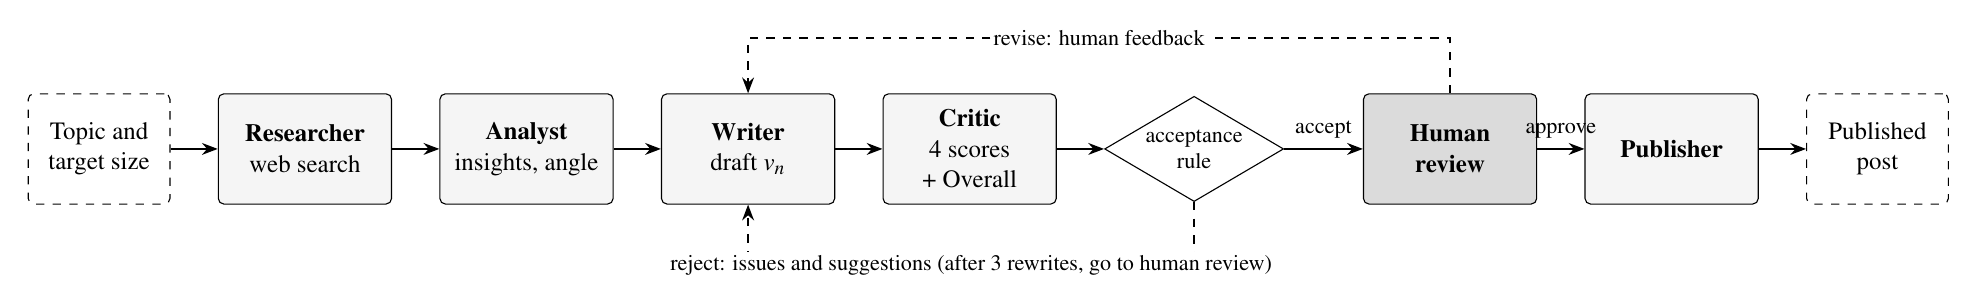
\begin{tikzpicture}[
  font=\small,
  node distance=6mm,
  agent/.style={draw, rounded corners=2pt, minimum width=22mm, minimum height=14mm, align=center, fill=gray!8},
  io/.style={draw, dashed, rounded corners=2pt, minimum width=18mm, minimum height=14mm, align=center},
  human/.style={agent, fill=gray!28},
  decision/.style={draw, diamond, aspect=1.7, align=center, inner sep=1pt, fill=white, font=\footnotesize},
  flow/.style={-{Stealth[length=2mm]}, thick},
  back/.style={-{Stealth[length=2mm]}, thick, dashed},
  lbl/.style={font=\footnotesize, fill=white, inner sep=1pt},
]
\node[io] (in) {Topic and\\target size};
\node[agent, right=of in] (res) {\textbf{Researcher}\\web search};
\node[agent, right=of res] (ana) {\textbf{Analyst}\\insights, angle};
\node[agent, right=of ana] (wri) {\textbf{Writer}\\draft $v_n$};
\node[agent, right=of wri] (cri) {\textbf{Critic}\\4 scores\\+ Overall};
\node[decision, right=of cri] (dec) {acceptance\\rule};
\node[human, right=10mm of dec] (hitl) {\textbf{Human}\\\textbf{review}};
\node[agent, right=of hitl] (pub) {\textbf{Publisher}};
\node[io, right=of pub] (out) {Published\\post};

\draw[flow] (in) -- (res);
\draw[flow] (res) -- (ana);
\draw[flow] (ana) -- (wri);
\draw[flow] (wri) -- (cri);
\draw[flow] (cri) -- (dec);
\draw[flow] (dec) -- node[above, font=\footnotesize] {accept} (hitl);
\draw[flow] (hitl) -- node[above, font=\footnotesize] {approve} (pub);
\draw[flow] (pub) -- (out);

\draw[back] (dec.south) -- ++(0,-8mm) -| node[lbl, pos=0.25] {reject: issues and suggestions (after 3 rewrites, go to human review)} (wri.south);
\draw[back] (hitl.north) -- ++(0,7mm) -| node[lbl, pos=0.25] {revise: human feedback} (wri.north);
\end{tikzpicture}}
\caption{Pipeline studied. Solid arrows show the main flow and dashed arrows the two revision paths. The Critic's acceptance rule is the automated gate evaluated in this paper; the human review precedes publication.}
\label{fig:architecture}
\end{figure*}

\textbf{Rubric.} The Critic scores each post on four dimensions from 1 (\emph{very poor}) to 5 (\emph{excellent}), with a verbal anchor for every point (Appendix, Table~\ref{tab:rubric}): \emph{Clarity and Readability} \cite{rooderkerk2016nocomment}, \emph{Relevance and Informational Value} and \emph{Professional Appropriateness} \cite{usera2026linkedin}, and \emph{Engagement Quality} \cite{usera2025predicts}. It then gives a holistic \emph{Overall Quality} score, last and without anchors, so that it follows from the dimension scores; Overall is not used by the acceptance rule. The Critic receives the topic and the post but not the sources, so factual accuracy is not assessed. Each issue the Critic reports is tagged with a dimension and a scale point, and a check in code lowers a score that is higher than the worst point cited for that dimension if the Critic does not resolve the contradiction when asked once. The same questions were given to the human raters.

\textbf{Acceptance rule.} The decision is computed in code, not elicited from the model, so that the same rule applies to any set of scores. A post is accepted when the composite $0.35\,\mathit{Cla} + 0.35\,\mathit{Rel} + 0.15\,\mathit{Pro} + 0.15\,\mathit{Eng}$ is at least 3.5 and no two dimensions score below 3 with at least one of them being Clarity or Relevance. Length, external links and engagement bait are checked separately and do not change the scores. This rule replaced one, fixed before data collection, that accepted a post when every dimension scored at least 3; that rule accepted all 22 development runs at the first pass, since 3 is anchored as \emph{acceptable}. The change was made on 8 September 2026, after the human data collection had started, and we report it as a deviation from the planned design. Both rules accept the ten posts on the scores analyzed here; applied to the scores given at generation time, however, the current rule would have rejected two of them (composites 3.15 and 3.35), which is why the posts reaching the human raters are those the earlier rule admitted.

% ═════════════════════════════════════════════════════════════════════════════
\section{\uppercase{Evaluation}}
\label{sec:evaluation}

The evaluation addresses four research questions:

\begin{itemize}
\item[\textbf{RQ1}] To what extent do the Critic's scores agree with human ratings of the same posts, beyond the agreement expected by chance?
\item[\textbf{RQ2}] How reliable are the human ratings of these posts?
\item[\textbf{RQ3}] How stable are the Critic's scores across repeated runs, and do they respond to a clear degradation of the posts?
\item[\textbf{RQ4}] Does the Critic distinguish posts written by different Writer models for the same topics, and how much do its scores depend on the wording of its own prompt?
\end{itemize}

\subsection{Posts, Raters and Procedure}
\label{sec:setup}

\textbf{Posts.} The corpus consists of \NPosts{} LinkedIn posts in Brazilian Portuguese generated by the pipeline between 29 August and 2 September 2026 for ten topics on work and software development (Appendix, Table~\ref{tab:posts}), with \CharMin{} to \CharMax{} characters. All ten were accepted by the Critic at the first pass, so the evaluated versions are first drafts; none was submitted to the human checkpoint. The Writer configuration changed during generation: seven posts were written by GPT-4o (\texttt{gpt-4o-2024-08-06}) and three (J, L and P) by GPT-4o-mini (\texttt{gpt-4o-mini-2024-07-18}). The ten posts were taken from a development corpus of 16 accepted posts; \TODO{state how the ten posts were selected}.

\textbf{Raters and questionnaire.} \NRaters{} raters completed the questionnaire between 3 and 8 September 2026. \TODO{recruitment procedure, background (profession, LinkedIn use), native language and consent/ethics procedure}. The questionnaire (Google Forms) showed, for each post, the requested topic and the post text, in the same order for all raters, followed by five mandatory items on a five-point scale \cite{likert1932technique,krosnick1999maximizing}: the four rubric questions given to the Critic and Overall Quality. \TODO{confirm whether the per-point anchors of Table~\ref{tab:rubric} were shown to the raters}. Raters were asked to judge each dimension independently and not to assess factual accuracy; the posts were not presented as AI-generated, and the Critic's scores were not disclosed. Each rater produced 50 ratings, 900 in total.

\textbf{Critic scores.} RQ1 and RQ2 use Critic scores produced for these post versions on 8 September 2026, in one run per post with the final Critic prompt; they replace neither the posts nor the earlier assessments made during generation (Section~\ref{sec:limitations}). For RQ3, the Critic was run \RepRuns{} more times on each post and once on a version truncated to its first 35\% of characters, cut back to the preceding word boundary (\RepCalls{} calls). In these calls the target size given to the Critic was the medium range for every post, including the three requested as small; the target size only enters the contextual notes of the prompt, not the rubric. These runs did not replace the stored scores.

\textbf{Writer benchmark (RQ4).} On 18 September 2026 the pipeline was run again on the same ten topics, with the same target sizes, once with Claude Sonnet 5 and once with Gemini 3.8 Flash as the Writer, giving ten posts per model; no run failed. Researcher, Analyst and Critic kept their models and temperatures, but the pipeline was not identical to the one that produced the human-rated corpus: all agent prompts had been translated to English (the output language remained Brazilian Portuguese), the Researcher and Analyst prompts were replaced by revised versions, the models were accessed through OpenRouter without dated snapshots, and the research step ran again for every post. The Critic prompt therefore changed as well (hash \BmNewHash{} instead of \BmOldHash{}), with the same rubric, anchors and acceptance rule. To compare the three Writers under one Critic, the ten human-rated posts were scored once more with the same Critic model (GPT-4.1, temperature 0.1) and the current prompt, without replacing the scores used in RQ1--RQ3; the two scores of the same text isolate the effect of the prompt revision. No human ratings were collected for the new posts.

\subsection{Metrics}
\label{sec:metrics}

For each dimension, the Critic is compared with each rater on each post (\NCHperDim{} comparisons per dimension) and every pair of raters on each post (\NHHperDim{} pairs). Exact agreement is the proportion of identical scores and within-one agreement the proportion differing by at most one point; four-dimension values are means over Clarity, Relevance, Professional Appropriateness and Engagement. Because percentage agreement is high whenever scores concentrate on few values, we also report the agreement expected by chance from the observed score distributions ($\sum_k p_k q_k$ for exact agreement) and that of a constant predictor outputting the most frequent human score. As chance-corrected and association measures we use the quadratic weighted kappa $\kappa_w$ \cite{cohen1968weighted}, Spearman's $\rho$ between the Critic score and the mean human score per post, and Krippendorff's ordinal $\alpha$ among raters \cite{krippendorff2018content}; score levels are compared through the mean difference (bias, Critic minus human). The sum of squares of each dimension is decomposed into rater and post components. Since posts and raters are the independent units, 95\% confidence intervals come from a percentile bootstrap resampling both \cite{efron1994bootstrap} (2,000 replicates; posts only for $\alpha$). As a sensitivity analysis defined after inspecting the data, the analysis is repeated without the \FlaggedN{} raters who gave the minimum score to at least half of their ratings. For RQ4, Writers are compared through mean scores and paired per-topic differences of the composite, with bootstrap intervals over posts; with one Critic run per post, these intervals exclude run-to-run variation.

\subsection{Results}

\begin{table*}[t]
\centering
\caption{Exact and within-one ($\pm1$) agreement between pairs of human raters, between the Critic and human raters, and expected by chance for Critic--human comparisons given the observed score distributions. Confidence intervals from the two-way bootstrap.}
\label{tab:agreement}
\small
\begin{tabular}{lcccccc}
\toprule
 & \multicolumn{2}{c}{Human--Human} & \multicolumn{2}{c}{Critic--Human} & \multicolumn{2}{c}{Chance (Critic--Human)} \\
\cmidrule(lr){2-3}\cmidrule(lr){4-5}\cmidrule(lr){6-7}
Dimension & Exact & $\pm1$ & Exact & $\pm1$ & Exact & $\pm1$ \\
\midrule
Clarity and Readability & 31.7\% & 71.0\% & 41.1\% & 89.4\% & 41.1\% & 89.4\% \\
Relevance and Informational Value & 26.9\% & 66.0\% & 21.7\% & 67.8\% & 20.4\% & 67.0\% \\
Professional Appropriateness & 30.1\% & 73.5\% & 42.2\% & 88.3\% & 41.8\% & 88.6\% \\
Engagement Quality & 25.2\% & 64.2\% & 22.2\% & 68.9\% & 24.1\% & 68.8\% \\
\midrule
\textbf{Four dimensions} & \textbf{28.4\%} & \textbf{68.7\%} & \textbf{31.8\%} & \textbf{78.6\%} & \textbf{31.9\%} & \textbf{78.4\%} \\
\quad 95\% CI & 21.0\%--36.5\% & 55.2\%--81.0\% & 22.8\%--40.8\% & 66.9\%--88.2\% & & \\
\midrule
Overall Quality & 27.1\% & 67.4\% & 23.3\% & 69.4\% & 24.0\% & 69.4\% \\
\bottomrule
\end{tabular}

\end{table*}

\begin{table*}[t]
\centering
\caption{Score levels and association. $M$ ($SD$): mean and standard deviation over all ratings; bias: Critic minus human; $\kappa_w$: quadratic weighted kappa; $\rho$: Spearman correlation between the Critic score and the mean human score per post ($n=10$; n/a when the Critic gave all posts the same score); $\alpha_H$: Krippendorff's ordinal alpha among human raters.}
\label{tab:scores}
\small
\begin{adjustbox}{max width=\textwidth}
\begin{tabular}{lccccccc}
\toprule
Dimension & Human $M$ ($SD$) & Critic $M$ ($SD$) & Bias [95\% CI] & MAE & $\kappa_w$ & $\rho$ & $\alpha_H$ \\
\midrule
Clarity and Readability & 3.91 (1.11) & 4.00 (0.00) & +0.09 [$-$0.26, +0.48] & 0.76 & 0.00 & n/a & $-$0.02 \\
Relevance and Informational Value & 3.74 (1.19) & 3.20 (0.42) & $-$0.54 [$-$0.98, $-$0.05] & 1.12 & 0.01 & 0.13 & $-$0.01 \\
Professional Appropriateness & 3.93 (1.07) & 4.10 (0.32) & +0.17 [$-$0.22, +0.56] & 0.75 & 0.05 & 0.53 & $-$0.01 \\
Engagement Quality & 3.66 (1.23) & 3.30 (0.48) & $-$0.36 [$-$0.84, +0.13] & 1.11 & 0.00 & 0.04 & $-$0.02 \\
\midrule
Overall Quality & 3.77 (1.12) & 3.20 (0.42) & $-$0.57 [$-$1.01, $-$0.09] & 1.09 & $-$0.02 & $-$0.22 & $-$0.03 \\
\bottomrule
\end{tabular}

\end{adjustbox}
\end{table*}

\subsubsection{Critic--Human Agreement (RQ1)}

Across the four dimensions, Critic--human exact agreement was \CHexAll{} (95\% CI \CHexLo{}--\CHexHi{}) and within-one agreement \CHwAll{} (\CHwLo{}--\CHwHi{}), against \HHexAll{} and \HHwAll{} for pairs of raters (Table~\ref{tab:agreement}). The agreement expected by chance from the score distributions was \CHchanceExAll{} for exact and \CHchanceWAll{} for within-one agreement; the observed minus chance difference lies between \ChanceDiffExLo{} and \ChanceDiffExHi{} percentage points for exact agreement (95\% CI). A constant predictor always outputting the most frequent human score, 4 in every dimension, would reach \ConstExAll{} exact agreement, more than the Critic. The differences between dimensions follow from where the Critic's scores fall: agreement is highest on Clarity (\CHexCla{}) and Professional Appropriateness (\CHexPro{}), where the Critic almost always gave 4, and lowest on Relevance (\CHexRel{}) and Engagement (\CHexEng{}), where it mostly gave 3. Consistently, $\kappa_w$ is close to zero in every dimension and the per-post correlation is weak or undefined (Table~\ref{tab:scores}).

\subsubsection{Reliability of Human Ratings (RQ2)}

Human raters did not agree with one another beyond chance either: human--human exact agreement (\HHexAll{}) matches its chance expectation (\HHchanceExAll{}), and Krippendorff's $\alpha$ lies between \AlphaMin{} and \AlphaMax{} in all dimensions. Differences between posts account for only \VarPostMin{}--\VarPostMax{} of the variation in human scores, against \VarRaterMin{}--\VarRaterMax{} for differences between raters; the mean human score of a post ranged only from \PostMeanMin{} to \PostMeanMax{}. A human score thus mainly reflects the rater's leniency, which leaves little between-post signal for the Critic to agree with. Score levels nevertheless differ: the Critic is close to the human mean on Clarity (bias \BiasCla{}) and Professional Appropriateness (\BiasPro{}) but stricter on Relevance (\BiasRel{}, 95\% CI \BiasLoRel{} to \BiasHiRel{}) and Overall Quality (\BiasOve{}, \BiasLoOve{} to \BiasHiOve{}), a severity applied almost identically to every post. Excluding the \FlaggedN{} raters with mostly minimum scores did not change these conclusions (Critic--human exact agreement \SensCHexAll{} against a chance expectation of \SensChanceExAll{}; $\alpha$ still close to zero).

\subsubsection{Critic Stability and Sensitivity (RQ3)}

\begin{table}[t]
\centering
\caption{Critic test--retest stability over \RepRuns{} repeated runs per post: mean within-post standard deviation, proportion of runs reproducing the stored score, and proportion of posts whose runs were all identical.}
\label{tab:repeat}
\begin{adjustbox}{max width=\columnwidth}
\begin{tabular}{lccc}
\toprule
Dimension & Within-post $SD$ & Runs = reported score & Posts with identical runs \\
\midrule
Clarity and Readability & 0.00 & 100.0\% & 100.0\% \\
Relevance and Informational Value & 0.00 & 100.0\% & 100.0\% \\
Professional Appropriateness & 0.05 & 86.0\% & 90.0\% \\
Engagement Quality & 0.04 & 92.0\% & 90.0\% \\
Overall Quality & 0.10 & 94.0\% & 80.0\% \\
\bottomrule
\end{tabular}

\end{adjustbox}
\end{table}

The Critic's scores were stable (Table~\ref{tab:repeat}): repeated runs reproduced the stored Clarity and Relevance scores in \RepEqualCla{} and \RepEqualRel{} of the cases, and the remaining variation never exceeded one point. The decision changed across runs for \RepFlips{} post (H), whose composite moved between 3.50 and 3.35. The Critic also responded to a clear degradation: \TruncReject{} of the truncated posts were rejected, with mean Engagement falling from \RepMeanEng{} to \TruncMeanEng{} and Clarity from \RepMeanCla{} to \TruncMeanCla{}, although Relevance changed little (\RepMeanRel{} to \TruncMeanRel{}). The low agreement in RQ1 is therefore not random Critic noise: the Critic is consistent and separates an intact post from a mutilated one, but gives nearly the same scores to all intact posts.

\subsubsection{Writer Comparison and Prompt Sensitivity (RQ4)}

\begin{figure*}[t]
\centering
% GERADO por study/analysis/benchmark.py — não editar à mão.
% Requer \usepackage{pgfplots} e \usepgfplotslibrary{groupplots}.
\definecolor{benchBlue}{HTML}{2A78D6}
\definecolor{benchOrange}{HTML}{EB6834}
\definecolor{benchAqua}{HTML}{1BAF7A}
\definecolor{benchGray}{HTML}{898781}
\begin{tikzpicture}
\begin{groupplot}[group style={group size=2 by 1, horizontal sep=1.6cm},
  height=5.2cm, axis line style={draw=black!45}, tick style={draw=black!45},
  tick label style={font=\footnotesize}, label style={font=\footnotesize},
  title style={font=\footnotesize\bfseries, yshift=-4pt},
  ymajorgrids, grid style={draw=black!10}, axis x line*=bottom, axis y line*=left]
\nextgroupplot[width=0.47\textwidth, title={(a) Mean score per dimension (current Critic)},
  ybar=1.2pt, bar width=5pt, ymin=1, ymax=5, ytick={1,2,3,4,5}, ylabel={Critic score},
  symbolic x coords={Cla,Rel,Pro,Eng,Ove}, xtick=data, enlarge x limits=0.14,
  legend style={font=\scriptsize, draw=none, fill=none, at={(0.5,-0.2)}, anchor=north, legend columns=3},
  legend image code/.code={\draw[#1, draw=none] (0cm,-0.08cm) rectangle (0.24cm,0.1cm);}]
\addplot[fill=benchBlue, draw=none, error bars/.cd, y dir=both, y explicit, error bar style={draw=black!55, line width=0.4pt}] coordinates {(Cla,4.000) += (0,0.000) -= (0,0.000) (Rel,3.200) += (0,0.300) -= (0,0.200) (Pro,4.300) += (0,0.300) -= (0,0.200) (Eng,3.300) += (0,0.300) -= (0,0.300) (Ove,3.300) += (0,0.300) -= (0,0.300)};
\addlegendentry{GPT-4o/4o-mini}
\addplot[fill=benchOrange, draw=none, error bars/.cd, y dir=both, y explicit, error bar style={draw=black!55, line width=0.4pt}] coordinates {(Cla,4.300) += (0,0.400) -= (0,0.400) (Rel,4.000) += (0,0.000) -= (0,0.000) (Pro,4.500) += (0,0.300) -= (0,0.300) (Eng,4.100) += (0,0.200) -= (0,0.100) (Ove,4.100) += (0,0.200) -= (0,0.100)};
\addlegendentry{Claude Sonnet 5}
\addplot[fill=benchAqua, draw=none, error bars/.cd, y dir=both, y explicit, error bar style={draw=black!55, line width=0.4pt}] coordinates {(Cla,4.600) += (0,0.300) -= (0,0.300) (Rel,4.000) += (0,0.000) -= (0,0.000) (Pro,5.000) += (0,0.000) -= (0,0.000) (Eng,4.000) += (0,0.000) -= (0,0.000) (Ove,4.000) += (0,0.000) -= (0,0.000)};
\addlegendentry{Gemini 3.8 Flash}
\nextgroupplot[width=0.47\textwidth, title={(b) Composite score per post},
  ymin=1.5, ymax=5, ytick={2,3,3.5,4,5}, yticklabels={2,3,3.5,4,5}, ylabel={Composite},
  symbolic x coords={A,C,D,E,F,H,I,J,L,P}, xtick=data, xlabel={Post (same topic across writers)}, enlarge x limits=0.06,
  legend style={font=\scriptsize, draw=none, fill=none, at={(0.5,-0.3)}, anchor=north, legend columns=2}]
\addplot[draw=black!60, line width=0.6pt, forget plot] coordinates {(A,3.5) (P,3.5)};
\node[font=\scriptsize, text=black!60, anchor=south east] at (axis cs:P,3.5) {acceptance threshold};
\addplot[only marks, mark=o, mark size=2.3pt, mark options={draw=benchGray, fill=white, line width=0.6pt}] coordinates {(A,3.65) (C,3.50) (D,4.00) (E,3.50) (F,3.50) (H,3.50) (I,3.50) (J,3.50) (L,3.65) (P,4.00)};
\addlegendentry{GPT-4o/4o-mini (original prompt)}
\addplot[only marks, mark=*, mark size=2.3pt, mark options={draw=white, fill=benchBlue, line width=0.6pt}] coordinates {(A,3.80) (C,3.50) (D,4.15) (E,3.50) (F,3.50) (H,3.50) (I,3.50) (J,3.50) (L,3.65) (P,4.00)};
\addlegendentry{GPT-4o/4o-mini}
\addplot[only marks, mark=square*, mark size=2.3pt, mark options={draw=white, fill=benchOrange, line width=0.6pt}] coordinates {(A,4.15) (C,4.15) (D,4.50) (E,4.50) (F,4.35) (H,4.15) (I,4.35) (J,4.00) (L,4.15) (P,3.65)};
\addlegendentry{Claude Sonnet 5}
\addplot[only marks, mark=triangle*, mark size=2.3pt, mark options={draw=white, fill=benchAqua, line width=0.6pt}] coordinates {(A,4.15) (C,4.50) (D,4.50) (E,4.50) (F,4.15) (H,4.15) (I,4.15) (J,4.50) (L,4.50) (P,4.50)};
\addlegendentry{Gemini 3.8 Flash}
\end{groupplot}
\end{tikzpicture}

\caption{Critic scores for the ten topics written by three Writers. (a) Mean score per dimension under the current Critic prompt, with 95\% bootstrap intervals over posts. (b) Composite score per post; the horizontal line is the acceptance threshold. Open gray circles are the original scores of the human-rated posts (prompt \BmOldHash{}); filled markers use the current prompt (\BmNewHash{}), so the distance between an open circle and the blue dot of the same post is the effect of the prompt revision alone. Exact values in Table~\ref{tab:benchmark}.}
\label{fig:benchmark}
\end{figure*}

\begin{table}[t]
\centering
\caption{Critic scores per Writer: accepted posts (Acc.), mean composite with 95\% bootstrap interval, and mean per dimension. The first row uses the original Critic prompt; the others share the current one.}
\label{tab:benchmark}
\begin{adjustbox}{max width=\columnwidth}
% GERADO por study/analysis/benchmark.py — não editar à mão.
\begin{tabular}{lcccccccc}
\toprule
Writer & Acc. & Composite [95\% CI] & Cla & Rel & Pro & Eng & Ove \\
\midrule
GPT-4o/4o-mini (original prompt) & 10/10 & 3.63 [3.53, 3.75] & 4.0 & 3.2 & 4.1 & 3.3 & 3.2 \\
\midrule
GPT-4o/4o-mini & 10/10 & 3.66 [3.53, 3.81] & 4.0 & 3.2 & 4.3 & 3.3 & 3.3 \\
Claude Sonnet 5 & 10/10 & 4.20 [4.03, 4.33] & 4.3 & 4.0 & 4.5 & 4.1 & 4.1 \\
Gemini 3.8 Flash & 10/10 & 4.36 [4.25, 4.46] & 4.6 & 4.0 & 5.0 & 4.0 & 4.0 \\
\bottomrule
\end{tabular}

\end{adjustbox}
\end{table}

Under the same Critic prompt, the Claude and Gemini posts scored higher than the human-rated GPT-4o/4o-mini posts in every dimension (Figure~\ref{fig:benchmark}a, Table~\ref{tab:benchmark}): the composite was \BmClaComp{} (95\% CI \BmClaCompLo{}--\BmClaCompHi{}) for Claude and \BmGemComp{} (\BmGemCompLo{}--\BmGemCompHi{}) for Gemini, against \BmGptComp{} (\BmGptCompLo{}--\BmGptCompHi{}) for GPT. Both were higher than GPT on \BmWinsClaGpt{} and \BmWinsGemGpt{} of the ten topics, respectively, with mean paired differences of \BmDiffClaGpt{} (\BmDiffClaGptLo{} to \BmDiffClaGptHi{}) and \BmDiffGemGpt{} (\BmDiffGemGptLo{} to \BmDiffGemGptHi{}). The acceptance decision, however, did not separate them: \BmClaAccept{}, \BmGemAccept{} and \BmGptAccept{} of the ten Claude, Gemini and GPT posts were accepted. Gemini and Claude were not distinguished (\BmDiffGemCla{}, \BmDiffGemClaLo{} to \BmDiffGemClaHi{}). Within each Writer the Critic again gave nearly constant scores: Relevance was 4 in \BmRelModeShare{} of the new posts, and the ten Gemini posts received only \BmGemVectors{} distinct combinations of the four scores.

The prompt revision had little effect on the human-rated posts (Figure~\ref{fig:benchmark}b, open circles versus blue dots). For the same ten texts, the mean change was \BmShiftComp{} on the composite, \BmShiftPro{} on Professional Appropriateness, \BmShiftClar{} on Clarity and \BmShiftRel{} on Relevance, and the number of changed decisions was \BmShiftDecisions{}.

% ═════════════════════════════════════════════════════════════════════════════
\section{\uppercase{Discussion}}
\label{sec:discussion}

Critic--human and human--human agreement percentages were similar, which could be read as evidence that the Critic judges like a human. Against the chance baseline that reading does not hold: both percentages are what independent scoring with the same score distributions produces. Three findings explain this and delimit what can be concluded.

\emph{The quality range was too narrow for agreement to be observable.} All posts came from the same pipeline and passed the Critic at the first pass, and the raters did not distinguish between them. The Critic behaved the same way: \CompAtThreshold{} of the ten posts obtained a composite of exactly 3.50, the threshold. Under such conditions no rater, human or automated, can agree beyond chance, and percentage agreement mainly reflects how close the typical scores of the two sources are. Validating a pipeline-embedded critic therefore requires items that span a meaningful quality range, for instance degraded or human-written posts added to the pipeline outputs, and a measured human reliability before critic--human agreement is interpreted.

\emph{The Critic is a stable, coarse filter rather than a ranker.} It rejects posts that lose most of their content and separates Writers whose outputs differ systematically, by about half a point on the composite, but within a set of competent posts it assigns nearly the same scores; Relevance, in particular, barely reacted to truncation and was 4 in \BmRelModeShare{} of the new posts. This is where the acceptance threshold operates, and the decision flip of post H shows that a one-point fluctuation suffices to change the outcome there. The Writer ranking should also be read with caution: it compares pipelines as much as models, no human rated the new posts, and it placed the GPT-family Writer last under a GPT-4.1 Critic, which at least does not suggest a preference for its own model family.

\emph{The Critic detects differences that the gate does not act on.} Its scores were robust to translating its prompt and changing its role description, which supports its use as a consistent measuring instrument. As a gate, however, it accepted every post of every Writer: the half-point gap between the GPT posts and the others lies entirely above the threshold, and nothing produced by the pipeline was rejected. A gate that passes all regular outputs contributes only its revision loop for clearly deficient drafts; its value for quality control depends on where the threshold sits relative to the range of outputs, which should be set from human judgments rather than from the Critic's own score distribution. For the architecture, these results argue against using Critic scores to rank posts or to skip human review. Robustness to the prompt was measured with the Critic model fixed; since the provenance hash covers the prompt but not the model, the model must be recorded and checked separately, as it is here.

\subsection{Limitations}
\label{sec:limitations}

The evaluation uses ten posts in a narrow quality range, all accepted at the first pass, so it says nothing about the Critic's behavior on rejected posts beyond the truncation control. The Critic scores analyzed in RQ1--RQ3 were produced after generation with the final prompt; the posts had been accepted during generation by an earlier version of the Critic prompt, whose scores differed in at least one dimension for five of the ten posts, although both versions accept all ten. In total, one Critic model (GPT-4.1) was used with three prompt versions, one language and one platform. The pipeline itself was not evaluated: there is no comparison with single-prompt generation or with the pipeline without the Critic, and the human checkpoint was not exercised. The Writer model was not constant in the human-rated corpus, and the Writer benchmark compares pipelines rather than isolated Writers, with one Critic run per post and no human ratings; the difference between Gemini and Claude is within sampling uncertainty. The raters are a convenience sample \TODO{describe}, and the conclusions concern these raters; all of them saw the posts in the same order, so fatigue is confounded with post identity. \TODO{if the per-point anchors were not shown to the raters, state here that the Critic and the raters did not use an identical instrument}. The acceptance rule was changed on the last day of the human data collection, although both rules accept all ten posts, and the rater exclusion criterion of the sensitivity analysis was defined after inspecting the data.

% ═════════════════════════════════════════════════════════════════════════════
\section{\uppercase{Conclusion}}
\label{sec:conclusion}

We asked whether an LLM critic embedded in a Human-in-the-Loop content pipeline is a reliable quality gate. Compared with \NRaters{} human raters on \NPosts{} pipeline-approved posts, the Critic's agreement did not exceed chance, and neither did the raters' agreement with one another. The Critic was stable, robust to a revision of its prompt and rejected mutilated posts, and it ranked three Writers by their average quality, but it gave nearly the same scores within each set of competent posts and accepted every post of every Writer. Evaluating a critic on the outputs of the pipeline it controls restricts the quality range until agreement statistics lose their meaning, and a critic that detects quality differences is not thereby a gate that acts on them. Future work will evaluate the Critic on corpora spanning the quality range, including human-rated posts from several Writers, compare the pipeline with and without the Critic on operational measures (revisions, human rejection rate, latency and cost), and use several Critic models and larger rater panels with randomized order. The prompts, the rubric and the analysis code are available at \TODO{anonymized repository URL}.

\section*{\uppercase{Acknowledgements}}

The authors acknowledge the use of an AI assistant to review the manuscript for grammar and style and to support the data analysis scripts. The authors are responsible for all the content, interpretations and conclusions presented in this paper.

\bibliographystyle{apalike}
{\small
\bibliography{refs}}

% ═════════════════════════════════════════════════════════════════════════════
\section*{\uppercase{Appendix}}

\begin{table*}[h]
\centering
\caption{Rubric used by the Critic and the human questionnaire (translated from Brazilian Portuguese). Scale labels: 1 very poor, 2 poor, 3 acceptable, 4 good, 5 excellent. Overall Quality (``All things considered, what is the overall quality of this post?'') has no per-point anchors.}
\label{tab:rubric}
\scriptsize
\setlength{\tabcolsep}{3pt}
\renewcommand{\arraystretch}{1.15}
\begin{tabularx}{\textwidth}{@{}>{\raggedright\arraybackslash}p{2.5cm}*{5}{>{\raggedright\arraybackslash}X}@{}}
\toprule
Dimension and question & 1 & 2 & 3 & 4 & 5 \\
\midrule
\textbf{Clarity and Readability.} Is the post clear, understandable, well structured and easy to read? &
Confusing. Dense block or overly long sentences; the central idea cannot be identified. &
Hard to follow. Weak structure, requires re-reading; the idea only appears at the end, or not at all. &
Understandable with average effort. Acceptable structure, but some passages are dense, truncated or repetitive. &
Clear and well organized. Fluent reading, central idea evident early, line breaks help. &
Exceptionally clear. Each paragraph advances the idea; rhythm and formatting serve the reader; nothing is superfluous. \\
\midrule
\textbf{Relevance and Informational Value.} Does the post deliver meaningful, substantive information appropriate for a professional audience and fulfil the intent of the topic? &
No value or off-topic. Informs nothing and/or does not address the intent of the topic. &
Generic. Common sense and broad claims without substance; only grazes the topic. &
Correct but predictable information. Covers the basics of the topic without adding much for people in the field. &
Substantive. Provides a data point, example or useful distinction and addresses the intent of the topic well. &
High value. Non-obvious, specific and actionable insight for the professional audience. \\
\midrule
\textbf{Professional Appropriateness.} Are the tone, language and presentation appropriate for a professional social network and the intended audience? &
Inappropriate. Offensive, sensationalist, jarringly informal or aggressively promotional. &
Out of place. Exaggeration, clickbait, empty marketing jargon, excessive emojis or punctuation. &
Acceptable. Nothing improper, but the register fluctuates or sounds impersonal and generic (``AI text''). &
Appropriate. Consistent and authentic professional tone; language suited to the audience. &
Exemplary. Credible and natural professional voice, calibrated to the audience, free of clichés. \\
\midrule
\textbf{Engagement Quality.} Does the post attract attention, sustain interest and encourage appropriate professional interaction? &
Does not hold attention. Opening without a hook and nothing to sustain reading, or an artificial request for interaction. &
Weak. Slow start and interest drops midway; generic invitation such as ``what do you think?''. &
Average. Functional opening, keeps the reader until the end; invitation present but not very specific. &
Good. Scroll-stopping opening, sustained interest, invitation anchored in the content of the post. &
Excellent. The first line compels reading on, tension is maintained, and the invitation draws on a specific experience of the reader. \\
\bottomrule
\end{tabularx}
\end{table*}

\begin{table*}[h]
\centering
\caption{Evaluated posts in questionnaire order: requested topic (translated), length in characters, stored Critic scores (Clarity, Relevance, Professional Appropriateness, Engagement, Overall) and mean human score per dimension.}
\label{tab:posts}
\footnotesize
\begin{tabular}{lp{6.2cm}rlccccc}
\toprule
 & & & & \multicolumn{5}{c}{Human mean} \\
\cmidrule(lr){5-9}
Post & Requested topic (translated) & Chars & Critic & Cl. & Rel. & Prof. & Eng. & Ov. \\
\midrule
A & What is technical debt and how can it be explained to non-technical people? & 896 & 4,3,4,4,3 & 4.2 & 3.9 & 4.0 & 3.7 & 4.0 \\
J & Junior programmers will no longer be hired from 2027 onwards & 1361 & 4,3,4,3,3 & 4.2 & 4.2 & 4.2 & 4.1 & 4.1 \\
D & Legacy code that nobody wants to touch and nobody manages to replace & 1867 & 4,4,4,4,4 & 3.9 & 3.8 & 4.1 & 3.7 & 3.7 \\
L & Why do retrospective meetings change nothing? & 1686 & 4,3,5,3,3 & 3.9 & 3.8 & 4.2 & 3.7 & 3.7 \\
F & Technical certifications have lost value in hiring processes & 1227 & 4,3,4,3,3 & 3.7 & 3.6 & 3.8 & 3.7 & 3.8 \\
P & A college degree is no longer of any use in the job market & 1197 & 4,4,4,4,4 & 3.8 & 3.8 & 3.7 & 3.6 & 3.7 \\
I & Artificial intelligence will transform the future of work & 1309 & 4,3,4,3,3 & 3.6 & 3.9 & 3.6 & 3.7 & 3.8 \\
E & How to double a development team's productivity in 30 days? & 938 & 4,3,4,3,3 & 3.8 & 3.4 & 3.8 & 3.3 & 3.6 \\
H & What is the future of programming? & 1555 & 4,3,4,3,3 & 3.7 & 3.4 & 3.7 & 3.4 & 3.5 \\
C & Daily stand-up meetings have become an empty ritual in most tech teams & 1183 & 4,3,4,3,3 & 4.2 & 3.7 & 4.1 & 3.7 & 3.8 \\
\bottomrule
\end{tabular}

\end{table*}

\end{document}
